\documentclass[a4paper, 14pt]{extarticle}

% Поля
%----------------------
\usepackage{geometry}
\geometry{a4paper,left=2cm,right=1cm,
    top=2cm,bottom=2cm,bindingoffset=0cm}
%----------------------

% Russian-specific packages
%----------------------
\usepackage[T2A]{fontenc}
\usepackage[utf8]{inputenc}
\usepackage[english, main=russian]{babel}
%----------------------

\usepackage{textcomp}

% Красная строка
%----------------------
\usepackage{indentfirst}
%----------------------

% Graphics
%----------------------
\usepackage{graphicx}
\graphicspath{ {./images} }
\usepackage{wrapfig}
%----------------------

% Import minted
%----------------------
\usepackage{minted}
%----------------------

\linespread{1.3}
\sloppy
\clubpenalty=10000
\widowpenalty=10000

\begin{document}

%--------------------------------------
%			ТИТУЛЬНЫЙ ЛИСТ
%--------------------------------------
\begin{titlepage}
\thispagestyle{empty}
\newpage


%Шапка титульного листа
%--------------------------------------
\vspace*{-60pt}
\hspace{-65pt}
\begin{minipage}{0.3\textwidth}
\hspace*{-20pt}\centering

\includegraphics[width=\textwidth]{emblem}
\end{minipage}
\begin{minipage}{0.67\textwidth}\small \textbf{
\vspace*{-0.7ex}
\hspace*{-6pt}\centerline{Министерство науки и высшего образования Российской Федерации}
\vspace*{-0.7ex}
\centerline{Федеральное государственное бюджетное образовательное учреждение }
\vspace*{-0.7ex}
\centerline{высшего образования}
\vspace*{-0.7ex}
\centerline{<<Московский государственный технический университет}
\vspace*{-0.7ex}
\centerline{имени Н.Э. Баумана}
\vspace*{-0.7ex}
\centerline{(национальный исследовательский университет)>>}
\vspace*{-0.7ex}
\centerline{(МГТУ им. Н.Э. Баумана)}}
\end{minipage}
%--------------------------------------

%Полосы
%--------------------------------------
\vspace{-25pt}
\hspace{-35pt}\rule{\textwidth}{2.3pt}

\vspace*{-20.3pt}
\hspace{-35pt}\rule{\textwidth}{0.4pt}
%--------------------------------------

\vspace{1.5ex}
\hspace{-35pt} \noindent \small ФАКУЛЬТЕТ\hspace{80pt} <<Информатика и системы управления>>

\vspace*{-16pt}
\hspace{47pt}\rule{0.83\textwidth}{0.4pt}

\vspace{0.5ex}
\hspace{-35pt} \noindent \small КАФЕДРА\hspace{50pt} <<Теоретическая информатика и компьютерные технологии>>

\vspace*{-16pt}
\hspace{30pt}\rule{0.866\textwidth}{0.4pt}
  
\vspace{11em}

\begin{center}
\Large {\bf Лабораторная работа № 6} \\ 
\large {\bf по курсу <<Языки и методы программирования>>} \\
\large <<Программа с графическим пользовательским интерфейсом>> \\
\large Вариант 3
\end{center}\normalsize

\vspace{8em}


\begin{flushright}
  {Студент группы ИУ9-22Б Павлов И. П. \hspace*{15pt}\\ 
  \vspace{2ex}
  Преподаватель Посевин Д. П.\hspace*{15pt}}
\end{flushright}

\bigskip

\vfill
 

\begin{center}
\textsl{Москва 2023}
\end{center}
\end{titlepage}
%--------------------------------------
%		КОНЕЦ ТИТУЛЬНОГО ЛИСТА
%--------------------------------------

\newpage
\section{Цель работы}
Приобретение навыков разработки программ с графическим пользовательским интерфейсом на основе библиотеки swing.

\section{Условие}
В течение лабораторной работы нужно разработать программу, рисующую на экране одно из изображений, перечисленных в таблицах 1 – 7. Программа должна иметь графический пользовательский интерфейс, через который пользователь может задавать параметры изображения. Изображение должно перерисовываться автоматически при изменении любого параметра.

Окружность радиуса r, изображённая с помощью квадратов со стороной a, наклоненных на угол \begin{math}\alpha\end{math}.

\section{Реализация класса CanvasPanel}
{\scriptsize
\begin{minted}{java}
import javax.swing.*;
import java.awt.*;
import java.lang.Math;
import java.util.ArrayList;

public class CanvasPanel extends JPanel {
    private Polygon hexagon;
    private Point center;
    private double angle;
    private int size;
    private ArrayList<Polygon> squares;

    public void setAngle(double angle) {
        this.angle = angle;
        repaint();
    }

    public void setSize(int size) {
        this.size = size;
        repaint();
    }

    public CanvasPanel() {
        this.center = new Point(getWidth() / 2, getHeight() / 2);
        this.angle = 0;
        this.size = 100;
        this.hexagon = createHexagon(center, size);
        this.squares = createSquares(hexagon, size);
    }

    @Override
    protected void paintComponent(Graphics g) {
        super.paintComponent(g);
        center = new Point(getWidth() / 2, getHeight() / 2);
        hexagon = createHexagon(center, size);
        squares = createSquares(hexagon, size);
        g.setColor(Color.BLACK);
        g.drawPolygon(hexagon);
        for (Polygon square : squares) {
            g.drawPolygon(square);
        }
    }

    private Polygon createHexagon(Point center, int size) {
        Polygon hexagon = new Polygon();
        for (int i = 0; i < 6; i++) {
            double angle_deg = 60 * i + angle;
            double angle_rad = Math.PI / 180 * angle_deg;
            int x = (int) (center.x + size * Math.cos(angle_rad));
            int y = (int) (center.y + size * Math.sin(angle_rad));
            hexagon.addPoint(x, y);
        }
        return hexagon;
    }

    private ArrayList<Polygon> createSquares(Polygon hexagon, int size) {
        ArrayList<Polygon> squares = new ArrayList<>();
        for (int i = 0; i < 6; i++) {
            Point p1 = new Point(hexagon.xpoints[i], hexagon.ypoints[i]);
            Point p2 = new Point(hexagon.xpoints[(i + 1) % 6], hexagon.ypoints[(i + 1) % 6]);
            Point diff = new Point(p2.x - p1.x, p2.y - p1.y);
            double angle_rad = Math.atan2(diff.y, diff.x);
            double x_offset = size * Math.sin(angle_rad);
            double y_offset = size * Math.cos(angle_rad);
            Point sq_p1 = new Point((int) (p1.x + x_offset), (int) (p1.y - y_offset));
            Point sq_p2 = new Point((int) (p2.x + x_offset), (int) (p2.y - y_offset));
            Point sq_p3 = new Point(p2.x, p2.y);
            Point sq_p4 = new Point(p1.x, p1.y);
            Polygon square = new Polygon();
            square.addPoint(sq_p1.x, sq_p1.y);
            square.addPoint(sq_p2.x, sq_p2.y);
            square.addPoint(sq_p3.x, sq_p3.y);
            square.addPoint(sq_p4.x, sq_p4.y);
            squares.add(square);
        }
        return squares;
    }

}
\end{minted}
}

\section{Реализация класса PictureForm}
{\scriptsize
\begin{minted}{java}
import javax.swing.*;
import javax.swing.event.ChangeEvent;
import javax.swing.event.ChangeListener;

public class PictureForm {
    private JPanel mainPanel;
    private JSlider rectangleSide;
    private JSlider rotationAngle;
    private CanvasPanel canvasPanel;


    public PictureForm () {
        rotationAngle.addChangeListener(new ChangeListener() {
            @Override
            public void stateChanged(ChangeEvent changeEvent) {
                double angle = rotationAngle.getValue();
                canvasPanel.setAngle(angle);
            }
        });

        rectangleSide.addChangeListener(new ChangeListener() {
            @Override
            public void stateChanged(ChangeEvent changeEvent) {
                int side = rectangleSide.getValue();
                canvasPanel.setSize(side);
            }
        });
    }

    public static void main(String[] args) {
        JFrame frame = new JFrame("Окружность");
        frame.setContentPane(new PictureForm().mainPanel);
        frame.setDefaultCloseOperation(JFrame.EXIT_ON_CLOSE);
        frame.pack();
        frame.setVisible(true);
    }
}
\end{minted}
}

\begin{figure}[h] 
\center{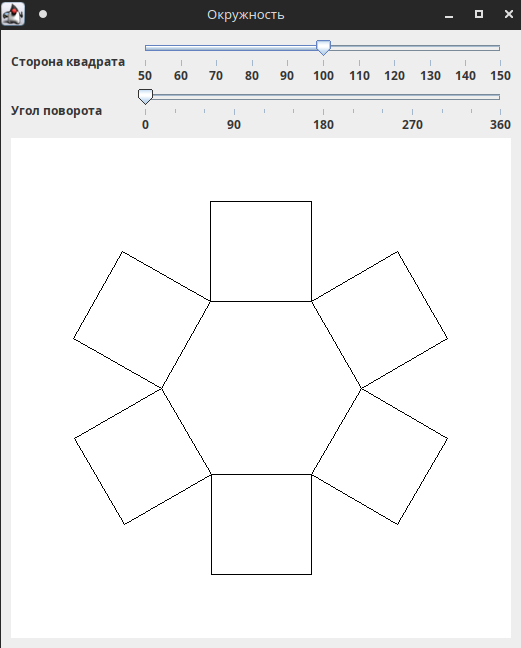
\includegraphics[scale=0.55]{output1.png}} 
\caption{Пример работы 1} 
\label{fig:image} 
\end{figure}

\begin{figure}[h] 
\center{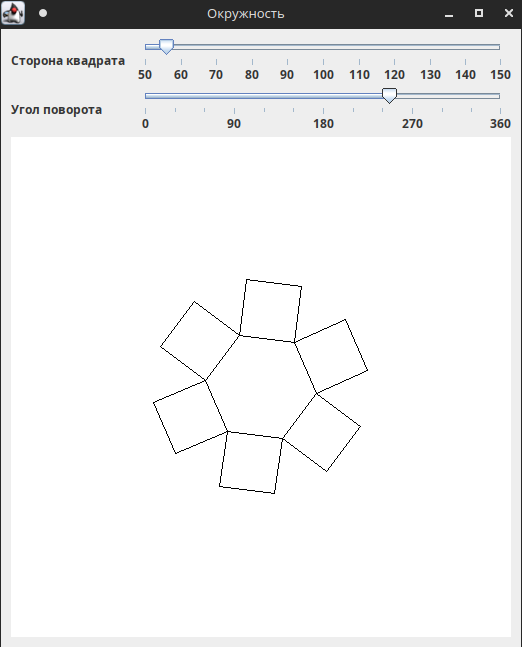
\includegraphics[scale=0.55]{output2.png}} 
\caption{Пример работы 2} 
\label{fig:image} 
\end{figure}

\begin{figure}[h] 
\center{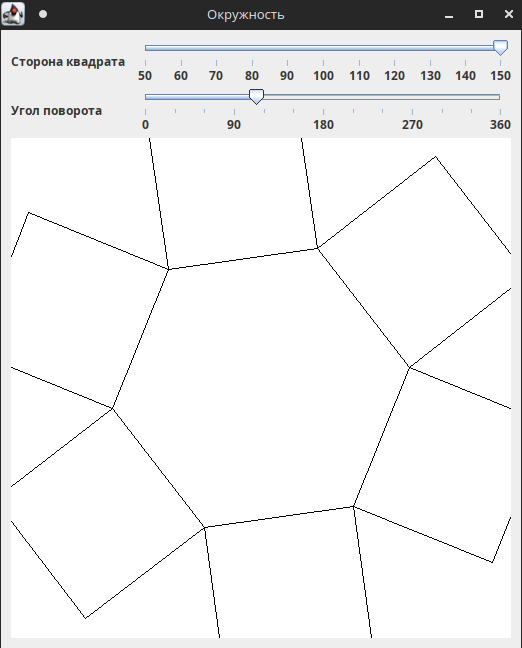
\includegraphics[scale=0.55]{output3.png}} 
\caption{Пример работы 3} 
\label{fig:image} 
\end{figure}

\end{document}
